% Editable vector source. From the tex directory, rebuild with:
% pdflatex -interaction=nonstopmode -halt-on-error -output-directory=figures/method-framework figures/method-framework/method-framework.tex
\documentclass[tikz,border=3mm]{standalone}
\usepackage[T1]{fontenc}
\usepackage{helvet}
\renewcommand{\familydefault}{\sfdefault}
\usetikzlibrary{arrows.meta,calc,shapes.misc}

\definecolor{ink}{HTML}{23374D}
\definecolor{inference}{HTML}{287F94}
\definecolor{training}{HTML}{C58539}
\definecolor{planneraccent}{HTML}{79659A}
\definecolor{modelaccent}{HTML}{698770}

% A hollow block head joins the two shaft outlines without a crossbar.
% Keep these dimensions in sync with flow: 3 pt interior + 0.8 pt borders.
\pgfdeclarearrow{
  name=HollowBlock,
  setup code={
    \pgfarrowssettipend{0.7pt}
    \pgfarrowssetbackend{-9pt}
    \pgfarrowssetlineend{-9pt}
    \pgfarrowshullpoint{0pt}{0pt}
    \pgfarrowshullpoint{-9pt}{6pt}
    \pgfarrowshullpoint{-9pt}{-6pt}
  },
  drawing code={
    \pgfsetlinewidth{0.8pt}
    \pgfsetinnerlinewidth{0pt}
    \pgfsetmiterjoin
    \pgfsetbuttcap
    \pgfsetfillcolor{white}
    \pgfpathmoveto{\pgfpoint{-9pt}{2.3pt}}
    \pgfpathlineto{\pgfpoint{-9pt}{6pt}}
    \pgfpathlineto{\pgfpoint{0pt}{0pt}}
    \pgfpathlineto{\pgfpoint{-9pt}{-6pt}}
    \pgfpathlineto{\pgfpoint{-9pt}{-2.3pt}}
    \pgfusepathqfillstroke
  }
}
\pgfdeclarearrow{
  name=HollowTail,
  setup code={
    \pgfarrowssettipend{0pt}
    \pgfarrowssetbackend{0pt}
    \pgfarrowssetlineend{0pt}
  },
  drawing code={
    \pgfsetlinewidth{0.8pt}
    \pgfsetinnerlinewidth{0pt}
    \pgfsetbuttcap
    \pgfpathmoveto{\pgfpoint{0pt}{-2.3pt}}
    \pgfpathlineto{\pgfpoint{0pt}{2.3pt}}
    \pgfusepathqstroke
  }
}

% Matched direction rings: a faint track and a gradually strengthening arc.
% Arguments: center coordinate, cycle color, label, direction (+1 or -1).
\newcommand{\drawcycle}[4]{%
  \draw[draw=#2!12,line width=0.8pt] (#1) circle[radius=1.08cm];
  \foreach \segment in {0,...,17} {
    \pgfmathsetmacro{\arcstart}{#4*(40+14*\segment)}
    \pgfmathsetmacro{\arcend}{#4*(40+14*(\segment+1)+0.3)}
    \pgfmathtruncatemacro{\arctint}{18+4*\segment}
    \draw[cycle stroke,draw=#2!\arctint]
      ($(#1)+(\arcstart:1.08cm)$)
      arc[start angle=\arcstart,end angle=\arcend,radius=1.08cm];
  }
  \pgfmathsetmacro{\headstart}{#4*292}
  \pgfmathsetmacro{\headend}{#4*332}
  \draw[cycle arrow,draw=#2]
    ($(#1)+(\headstart:1.08cm)$)
    arc[start angle=\headstart,end angle=\headend,radius=1.08cm];
  \node[cycle label,text=#2!85!black] at (#1) {#3\\cycle};
}

\begin{document}
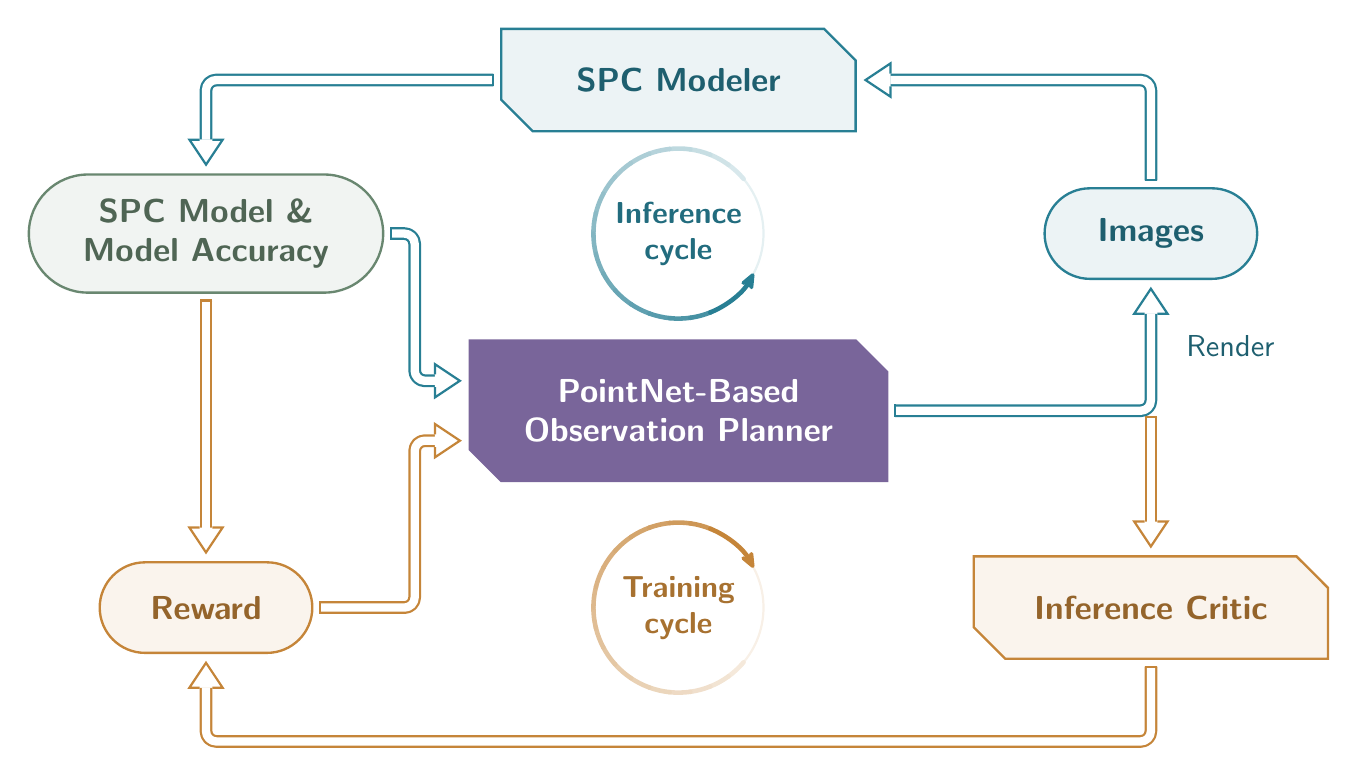
\begin{tikzpicture}[
  font=\sffamily,
  card/.style={
    line width=0.85pt, align=center,
    font=\fontsize{11.5}{14}\selectfont\bfseries,
    text=ink,outer sep=0.6pt
  },
  tone/.style={draw=#1,fill=#1!9,text=#1!75!black},
  module/.style={card,chamfered rectangle,
    chamfered rectangle corners={north east,south west},
    chamfered rectangle xsep=2mm,chamfered rectangle ysep=2mm,
    minimum width=4.1cm,minimum height=1.3cm,
    text width=3.3cm,inner xsep=4mm,inner ysep=3mm},
  data/.style={card,rounded rectangle,
    rounded rectangle arc length=180,
    minimum width=3cm,minimum height=1.15cm,
    inner xsep=1.5mm,inner ysep=2mm},
  flow/.style={line width=0.8pt,double=white,double distance=3pt,
    line cap=butt,line join=round,rounded corners=1.3mm,
    shorten <=0.8mm,shorten >=0.8mm,
    arrows={HollowTail-HollowBlock}},
  inference flow/.style={flow,draw=inference},
  training flow/.style={flow,draw=training},
  cycle stroke/.style={line width=1.65pt,line cap=round},
  cycle arrow/.style={cycle stroke,
    -{Stealth[length=2.8mm,width=2.25mm,round]}},
  cycle label/.style={font=\fontsize{10.5}{13}\selectfont\bfseries,
    align=center}
]

% Compact processing cards; color identifies each cycle or shared component.
\node[module,tone=planneraccent,fill=planneraccent,text=white,
  text width=4.1cm,minimum width=4.9cm,minimum height=1.65cm]
  (planner) at (0,0)
  {\mbox{PointNet-Based}\\Observation Planner};
\node[module,tone=inference] (modeler) at (0,4.2) {SPC Modeler};
\node[module,tone=training] (critic) at (6,-2.5) {Inference Critic};

% Flat capsules retain straight sides and avoid oversized elliptical outlines.
\node[data,tone=modelaccent,minimum width=4.8cm,minimum height=1.5cm]
  (model) at (-6,2.25) {SPC Model \&\\Model Accuracy};
\node[data,tone=inference] (images) at (6,2.25) {Images};
\node[data,tone=training] (reward) at (-6,-2.5) {Reward};

% Render sits to the right of the vertical planner-to-images segment.
% The unmarked bend also supplies the training critic.
\coordinate (render) at (6,0);
\draw[inference flow] (planner.east)
  -- (render)
  -- node[midway,right=3.2mm,font=\fontsize{10.5}{12}\selectfont,
    text=inference!75!black] {Render} (images.south);

% Inference: planner -> images -> SPC -> model/accuracy -> planner.
\draw[inference flow] (images.north) |- (modeler.east);
\draw[inference flow] (modeler.west) -| (model.north);
\draw[inference flow] (model.east)
  -- (-3.35,2.25) -- (-3.35,0.38)
  -- ([yshift=3.8mm]planner.west);

% Training: the critic and model accuracy supply reward feedback.
\draw[training flow] (render) -- (critic.north);
\draw[training flow] (critic.south)
  -- (6,-4.2) -- (-6,-4.2) -- (reward.south);
\draw[training flow] (model.south) -- (reward.north);
\draw[training flow] (reward.east)
  -- (-3.35,-2.5) -- (-3.35,-0.38)
  -- ([yshift=-3.8mm]planner.west);

% Circular direction markers surround the labels in the two open centers.
% Inference turns counterclockwise; training turns clockwise.
\coordinate (inference-cycle) at (0,2.25);
\drawcycle{inference-cycle}{inference}{Inference}{1}

\coordinate (training-cycle) at (0,-2.5);
\drawcycle{training-cycle}{training}{Training}{-1}

\end{tikzpicture}
\end{document}
